% Options for packages loaded elsewhere
% Options for packages loaded elsewhere
\PassOptionsToPackage{unicode}{hyperref}
\PassOptionsToPackage{hyphens}{url}
\PassOptionsToPackage{dvipsnames,svgnames,x11names}{xcolor}
%
\documentclass[
  letterpaper,
  DIV=11,
  numbers=noendperiod]{scrartcl}
\usepackage{xcolor}
\usepackage{amsmath,amssymb}
\setcounter{secnumdepth}{-\maxdimen} % remove section numbering
\usepackage{iftex}
\ifPDFTeX
  \usepackage[T1]{fontenc}
  \usepackage[utf8]{inputenc}
  \usepackage{textcomp} % provide euro and other symbols
\else % if luatex or xetex
  \usepackage{unicode-math} % this also loads fontspec
  \defaultfontfeatures{Scale=MatchLowercase}
  \defaultfontfeatures[\rmfamily]{Ligatures=TeX,Scale=1}
\fi
\usepackage{lmodern}
\ifPDFTeX\else
  % xetex/luatex font selection
\fi
% Use upquote if available, for straight quotes in verbatim environments
\IfFileExists{upquote.sty}{\usepackage{upquote}}{}
\IfFileExists{microtype.sty}{% use microtype if available
  \usepackage[]{microtype}
  \UseMicrotypeSet[protrusion]{basicmath} % disable protrusion for tt fonts
}{}
\makeatletter
\@ifundefined{KOMAClassName}{% if non-KOMA class
  \IfFileExists{parskip.sty}{%
    \usepackage{parskip}
  }{% else
    \setlength{\parindent}{0pt}
    \setlength{\parskip}{6pt plus 2pt minus 1pt}}
}{% if KOMA class
  \KOMAoptions{parskip=half}}
\makeatother
% Make \paragraph and \subparagraph free-standing
\makeatletter
\ifx\paragraph\undefined\else
  \let\oldparagraph\paragraph
  \renewcommand{\paragraph}{
    \@ifstar
      \xxxParagraphStar
      \xxxParagraphNoStar
  }
  \newcommand{\xxxParagraphStar}[1]{\oldparagraph*{#1}\mbox{}}
  \newcommand{\xxxParagraphNoStar}[1]{\oldparagraph{#1}\mbox{}}
\fi
\ifx\subparagraph\undefined\else
  \let\oldsubparagraph\subparagraph
  \renewcommand{\subparagraph}{
    \@ifstar
      \xxxSubParagraphStar
      \xxxSubParagraphNoStar
  }
  \newcommand{\xxxSubParagraphStar}[1]{\oldsubparagraph*{#1}\mbox{}}
  \newcommand{\xxxSubParagraphNoStar}[1]{\oldsubparagraph{#1}\mbox{}}
\fi
\makeatother

\usepackage{color}
\usepackage{fancyvrb}
\newcommand{\VerbBar}{|}
\newcommand{\VERB}{\Verb[commandchars=\\\{\}]}
\DefineVerbatimEnvironment{Highlighting}{Verbatim}{commandchars=\\\{\}}
% Add ',fontsize=\small' for more characters per line
\usepackage{framed}
\definecolor{shadecolor}{RGB}{241,243,245}
\newenvironment{Shaded}{\begin{snugshade}}{\end{snugshade}}
\newcommand{\AlertTok}[1]{\textcolor[rgb]{0.68,0.00,0.00}{#1}}
\newcommand{\AnnotationTok}[1]{\textcolor[rgb]{0.37,0.37,0.37}{#1}}
\newcommand{\AttributeTok}[1]{\textcolor[rgb]{0.40,0.45,0.13}{#1}}
\newcommand{\BaseNTok}[1]{\textcolor[rgb]{0.68,0.00,0.00}{#1}}
\newcommand{\BuiltInTok}[1]{\textcolor[rgb]{0.00,0.23,0.31}{#1}}
\newcommand{\CharTok}[1]{\textcolor[rgb]{0.13,0.47,0.30}{#1}}
\newcommand{\CommentTok}[1]{\textcolor[rgb]{0.37,0.37,0.37}{#1}}
\newcommand{\CommentVarTok}[1]{\textcolor[rgb]{0.37,0.37,0.37}{\textit{#1}}}
\newcommand{\ConstantTok}[1]{\textcolor[rgb]{0.56,0.35,0.01}{#1}}
\newcommand{\ControlFlowTok}[1]{\textcolor[rgb]{0.00,0.23,0.31}{\textbf{#1}}}
\newcommand{\DataTypeTok}[1]{\textcolor[rgb]{0.68,0.00,0.00}{#1}}
\newcommand{\DecValTok}[1]{\textcolor[rgb]{0.68,0.00,0.00}{#1}}
\newcommand{\DocumentationTok}[1]{\textcolor[rgb]{0.37,0.37,0.37}{\textit{#1}}}
\newcommand{\ErrorTok}[1]{\textcolor[rgb]{0.68,0.00,0.00}{#1}}
\newcommand{\ExtensionTok}[1]{\textcolor[rgb]{0.00,0.23,0.31}{#1}}
\newcommand{\FloatTok}[1]{\textcolor[rgb]{0.68,0.00,0.00}{#1}}
\newcommand{\FunctionTok}[1]{\textcolor[rgb]{0.28,0.35,0.67}{#1}}
\newcommand{\ImportTok}[1]{\textcolor[rgb]{0.00,0.46,0.62}{#1}}
\newcommand{\InformationTok}[1]{\textcolor[rgb]{0.37,0.37,0.37}{#1}}
\newcommand{\KeywordTok}[1]{\textcolor[rgb]{0.00,0.23,0.31}{\textbf{#1}}}
\newcommand{\NormalTok}[1]{\textcolor[rgb]{0.00,0.23,0.31}{#1}}
\newcommand{\OperatorTok}[1]{\textcolor[rgb]{0.37,0.37,0.37}{#1}}
\newcommand{\OtherTok}[1]{\textcolor[rgb]{0.00,0.23,0.31}{#1}}
\newcommand{\PreprocessorTok}[1]{\textcolor[rgb]{0.68,0.00,0.00}{#1}}
\newcommand{\RegionMarkerTok}[1]{\textcolor[rgb]{0.00,0.23,0.31}{#1}}
\newcommand{\SpecialCharTok}[1]{\textcolor[rgb]{0.37,0.37,0.37}{#1}}
\newcommand{\SpecialStringTok}[1]{\textcolor[rgb]{0.13,0.47,0.30}{#1}}
\newcommand{\StringTok}[1]{\textcolor[rgb]{0.13,0.47,0.30}{#1}}
\newcommand{\VariableTok}[1]{\textcolor[rgb]{0.07,0.07,0.07}{#1}}
\newcommand{\VerbatimStringTok}[1]{\textcolor[rgb]{0.13,0.47,0.30}{#1}}
\newcommand{\WarningTok}[1]{\textcolor[rgb]{0.37,0.37,0.37}{\textit{#1}}}

\usepackage{longtable,booktabs,array}
\usepackage{calc} % for calculating minipage widths
% Correct order of tables after \paragraph or \subparagraph
\usepackage{etoolbox}
\makeatletter
\patchcmd\longtable{\par}{\if@noskipsec\mbox{}\fi\par}{}{}
\makeatother
% Allow footnotes in longtable head/foot
\IfFileExists{footnotehyper.sty}{\usepackage{footnotehyper}}{\usepackage{footnote}}
\makesavenoteenv{longtable}
\usepackage{graphicx}
\makeatletter
\newsavebox\pandoc@box
\newcommand*\pandocbounded[1]{% scales image to fit in text height/width
  \sbox\pandoc@box{#1}%
  \Gscale@div\@tempa{\textheight}{\dimexpr\ht\pandoc@box+\dp\pandoc@box\relax}%
  \Gscale@div\@tempb{\linewidth}{\wd\pandoc@box}%
  \ifdim\@tempb\p@<\@tempa\p@\let\@tempa\@tempb\fi% select the smaller of both
  \ifdim\@tempa\p@<\p@\scalebox{\@tempa}{\usebox\pandoc@box}%
  \else\usebox{\pandoc@box}%
  \fi%
}
% Set default figure placement to htbp
\def\fps@figure{htbp}
\makeatother





\setlength{\emergencystretch}{3em} % prevent overfull lines

\providecommand{\tightlist}{%
  \setlength{\itemsep}{0pt}\setlength{\parskip}{0pt}}



 


\KOMAoption{captions}{tableheading}
\makeatletter
\@ifpackageloaded{tcolorbox}{}{\usepackage[skins,breakable]{tcolorbox}}
\@ifpackageloaded{fontawesome5}{}{\usepackage{fontawesome5}}
\definecolor{quarto-callout-color}{HTML}{909090}
\definecolor{quarto-callout-note-color}{HTML}{0758E5}
\definecolor{quarto-callout-important-color}{HTML}{CC1914}
\definecolor{quarto-callout-warning-color}{HTML}{EB9113}
\definecolor{quarto-callout-tip-color}{HTML}{00A047}
\definecolor{quarto-callout-caution-color}{HTML}{FC5300}
\definecolor{quarto-callout-color-frame}{HTML}{acacac}
\definecolor{quarto-callout-note-color-frame}{HTML}{4582ec}
\definecolor{quarto-callout-important-color-frame}{HTML}{d9534f}
\definecolor{quarto-callout-warning-color-frame}{HTML}{f0ad4e}
\definecolor{quarto-callout-tip-color-frame}{HTML}{02b875}
\definecolor{quarto-callout-caution-color-frame}{HTML}{fd7e14}
\makeatother
\makeatletter
\@ifpackageloaded{caption}{}{\usepackage{caption}}
\AtBeginDocument{%
\ifdefined\contentsname
  \renewcommand*\contentsname{Table of contents}
\else
  \newcommand\contentsname{Table of contents}
\fi
\ifdefined\listfigurename
  \renewcommand*\listfigurename{List of Figures}
\else
  \newcommand\listfigurename{List of Figures}
\fi
\ifdefined\listtablename
  \renewcommand*\listtablename{List of Tables}
\else
  \newcommand\listtablename{List of Tables}
\fi
\ifdefined\figurename
  \renewcommand*\figurename{Figure}
\else
  \newcommand\figurename{Figure}
\fi
\ifdefined\tablename
  \renewcommand*\tablename{Table}
\else
  \newcommand\tablename{Table}
\fi
}
\@ifpackageloaded{float}{}{\usepackage{float}}
\floatstyle{ruled}
\@ifundefined{c@chapter}{\newfloat{codelisting}{h}{lop}}{\newfloat{codelisting}{h}{lop}[chapter]}
\floatname{codelisting}{Listing}
\newcommand*\listoflistings{\listof{codelisting}{List of Listings}}
\usepackage{amsthm}
\theoremstyle{remark}
\AtBeginDocument{\renewcommand*{\proofname}{Proof}}
\newtheorem*{remark}{Remark}
\newtheorem*{solution}{Solution}
\newtheorem{refremark}{Remark}[section]
\newtheorem{refsolution}{Solution}[section]
\makeatother
\makeatletter
\makeatother
\makeatletter
\@ifpackageloaded{caption}{}{\usepackage{caption}}
\@ifpackageloaded{subcaption}{}{\usepackage{subcaption}}
\makeatother
\usepackage{bookmark}
\IfFileExists{xurl.sty}{\usepackage{xurl}}{} % add URL line breaks if available
\urlstyle{same}
\hypersetup{
  pdftitle={Storing Multiple Values in Lists},
  colorlinks=true,
  linkcolor={blue},
  filecolor={Maroon},
  citecolor={Blue},
  urlcolor={Blue},
  pdfcreator={LaTeX via pandoc}}


\title{Storing Multiple Values in Lists}
\author{}
\date{}
\begin{document}
\maketitle


\begin{itemize}
\tightlist
\item
  Explain what a list is.
\item
  Create and index lists of simple values.
\item
  Change the values of individual elements
\item
  Append values to an existing list
\item
  Reorder and slice list elements
\item
  Create and manipulate nested lists
\end{itemize}

\begin{itemize}
\tightlist
\item
  How can I store many values together?
\end{itemize}

In the previous episode, we analyzed a single file of clinical trial
inflammation data. However, after finding some peculiar and potentially
suspicious trends in the trial data we ask Dr.~Maverick if they have
performed any other clinical trials. Surprisingly, they say that they
have and provide us with 11 more CSV files for a further 11 clinical
trials they have undertaken since the initial trial.

Our goal now is to process all the inflammation data we have, which
means that we still have eleven more files to go!

The natural first step is to collect the names of all the files that we
have to process. In Python, a list is a way to store multiple values
together. In this episode, we will learn how to store multiple values in
a list as well as how to work with lists.

\subsection{Python lists}\label{python-lists}

Unlike NumPy arrays, lists are built into the language so we do not have
to load a library to use them. We create a list by putting values inside
square brackets and separating the values with commas:

\begin{Shaded}
\begin{Highlighting}[]
\NormalTok{odds }\OperatorTok{=}\NormalTok{ [}\DecValTok{1}\NormalTok{, }\DecValTok{3}\NormalTok{, }\DecValTok{5}\NormalTok{, }\DecValTok{7}\NormalTok{]}
\BuiltInTok{print}\NormalTok{(}\StringTok{\textquotesingle{}odds are:\textquotesingle{}}\NormalTok{, odds)}
\end{Highlighting}
\end{Shaded}

\begin{Shaded}
\begin{Highlighting}[]
\NormalTok{odds are: [1, 3, 5, 7]}
\end{Highlighting}
\end{Shaded}

We can access elements of a list using indices -- numbered positions of
elements in the list. These positions are numbered starting at 0, so the
first element has an index of 0.

\begin{Shaded}
\begin{Highlighting}[]
\BuiltInTok{print}\NormalTok{(}\StringTok{\textquotesingle{}first element:\textquotesingle{}}\NormalTok{, odds[}\DecValTok{0}\NormalTok{])}
\BuiltInTok{print}\NormalTok{(}\StringTok{\textquotesingle{}last element:\textquotesingle{}}\NormalTok{, odds[}\DecValTok{3}\NormalTok{])}
\BuiltInTok{print}\NormalTok{(}\StringTok{\textquotesingle{}"{-}1" element:\textquotesingle{}}\NormalTok{, odds[}\OperatorTok{{-}}\DecValTok{1}\NormalTok{])}
\end{Highlighting}
\end{Shaded}

\begin{Shaded}
\begin{Highlighting}[]
\NormalTok{first element: 1}
\NormalTok{last element: 7}
\NormalTok{"{-}1" element: 7}
\end{Highlighting}
\end{Shaded}

Yes, we can use negative numbers as indices in Python. When we do so,
the index \texttt{-1} gives us the last element in the list, \texttt{-2}
the second to last, and so on. Because of this, \texttt{odds{[}3{]}} and
\texttt{odds{[}-1{]}} point to the same element here.

There is one important difference between lists and strings: we can
change the values in a list, but we cannot change individual characters
in a string. For example:

\begin{Shaded}
\begin{Highlighting}[]
\NormalTok{names }\OperatorTok{=}\NormalTok{ [}\StringTok{\textquotesingle{}Curie\textquotesingle{}}\NormalTok{, }\StringTok{\textquotesingle{}Darwing\textquotesingle{}}\NormalTok{, }\StringTok{\textquotesingle{}Turing\textquotesingle{}}\NormalTok{]  }\CommentTok{\# typo in Darwin\textquotesingle{}s name}
\BuiltInTok{print}\NormalTok{(}\StringTok{\textquotesingle{}names is originally:\textquotesingle{}}\NormalTok{, names)}
\NormalTok{names[}\DecValTok{1}\NormalTok{] }\OperatorTok{=} \StringTok{\textquotesingle{}Darwin\textquotesingle{}}  \CommentTok{\# correct the name}
\BuiltInTok{print}\NormalTok{(}\StringTok{\textquotesingle{}final value of names:\textquotesingle{}}\NormalTok{, names)}
\end{Highlighting}
\end{Shaded}

\begin{Shaded}
\begin{Highlighting}[]
\NormalTok{names is originally: [\textquotesingle{}Curie\textquotesingle{}, \textquotesingle{}Darwing\textquotesingle{}, \textquotesingle{}Turing\textquotesingle{}]}
\NormalTok{final value of names: [\textquotesingle{}Curie\textquotesingle{}, \textquotesingle{}Darwin\textquotesingle{}, \textquotesingle{}Turing\textquotesingle{}]}
\end{Highlighting}
\end{Shaded}

works, but:

\begin{Shaded}
\begin{Highlighting}[]
\NormalTok{name }\OperatorTok{=} \StringTok{\textquotesingle{}Darwin\textquotesingle{}}
\NormalTok{name[}\DecValTok{0}\NormalTok{] }\OperatorTok{=} \StringTok{\textquotesingle{}d\textquotesingle{}}
\end{Highlighting}
\end{Shaded}

\begin{Shaded}
\begin{Highlighting}[]
\NormalTok{{-}{-}{-}{-}{-}{-}{-}{-}{-}{-}{-}{-}{-}{-}{-}{-}{-}{-}{-}{-}{-}{-}{-}{-}{-}{-}{-}{-}{-}{-}{-}{-}{-}{-}{-}{-}{-}{-}{-}{-}{-}{-}{-}{-}{-}{-}{-}{-}{-}{-}{-}{-}{-}{-}{-}{-}{-}{-}{-}{-}{-}{-}{-}{-}{-}{-}{-}{-}{-}{-}{-}{-}{-}{-}{-}}
\NormalTok{TypeError                                 Traceback (most recent call last)}
\NormalTok{\textless{}ipython{-}input{-}8{-}220df48aeb2e\textgreater{} in \textless{}module\textgreater{}()}
\NormalTok{      1 name = \textquotesingle{}Darwin\textquotesingle{}}
\NormalTok{{-}{-}{-}{-}\textgreater{} 2 name[0] = \textquotesingle{}d\textquotesingle{}}

\NormalTok{TypeError: \textquotesingle{}str\textquotesingle{} object does not support item assignment}
\end{Highlighting}
\end{Shaded}

does not.

\begin{tcolorbox}[enhanced jigsaw, bottomrule=.15mm, rightrule=.15mm, colback=white, colframe=quarto-callout-color-frame, leftrule=.75mm, arc=.35mm, breakable, toprule=.15mm, left=2mm, opacityback=0]

\vspace{-3mm}\textbf{Ch-Ch-Ch-Ch-Changes}\vspace{3mm}

Data which can be modified in place is called
\href{../learners/reference.md\#mutable}{mutable}, while data which
cannot be modified is called
\href{../learners/reference.md\#immutable}{immutable}. Strings and
numbers are immutable. This does not mean that variables with string or
number values are constants, but when we want to change the value of a
string or number variable, we can only replace the old value with a
completely new value.

Lists and arrays, on the other hand, are mutable: we can modify them
after they have been created. We can change individual elements, append
new elements, or reorder the whole list. For some operations, like
sorting, we can choose whether to use a function that modifies the data
in-place or a function that returns a modified copy and leaves the
original unchanged.

Be careful when modifying data in-place. If two variables refer to the
same list, and you modify the list value, it will change for both
variables!

\begin{Shaded}
\begin{Highlighting}[]
\NormalTok{mild\_salsa }\OperatorTok{=}\NormalTok{ [}\StringTok{\textquotesingle{}peppers\textquotesingle{}}\NormalTok{, }\StringTok{\textquotesingle{}onions\textquotesingle{}}\NormalTok{, }\StringTok{\textquotesingle{}cilantro\textquotesingle{}}\NormalTok{, }\StringTok{\textquotesingle{}tomatoes\textquotesingle{}}\NormalTok{]}
\NormalTok{hot\_salsa }\OperatorTok{=}\NormalTok{ mild\_salsa        }\CommentTok{\# \textless{}{-}{-} mild\_salsa and hot\_salsa point to the *same* list data in memory}
\NormalTok{hot\_salsa[}\DecValTok{0}\NormalTok{] }\OperatorTok{=} \StringTok{\textquotesingle{}hot peppers\textquotesingle{}}
\BuiltInTok{print}\NormalTok{(}\StringTok{\textquotesingle{}Ingredients in mild salsa:\textquotesingle{}}\NormalTok{, mild\_salsa)}
\BuiltInTok{print}\NormalTok{(}\StringTok{\textquotesingle{}Ingredients in hot salsa:\textquotesingle{}}\NormalTok{, hot\_salsa)}
\end{Highlighting}
\end{Shaded}

\begin{Shaded}
\begin{Highlighting}[]
\NormalTok{Ingredients in mild salsa: [\textquotesingle{}hot peppers\textquotesingle{}, \textquotesingle{}onions\textquotesingle{}, \textquotesingle{}cilantro\textquotesingle{}, \textquotesingle{}tomatoes\textquotesingle{}]}
\NormalTok{Ingredients in hot salsa: [\textquotesingle{}hot peppers\textquotesingle{}, \textquotesingle{}onions\textquotesingle{}, \textquotesingle{}cilantro\textquotesingle{}, \textquotesingle{}tomatoes\textquotesingle{}]}
\end{Highlighting}
\end{Shaded}

If you want variables with mutable values to be independent, you must
make a copy of the value when you assign it.

\begin{Shaded}
\begin{Highlighting}[]
\NormalTok{mild\_salsa }\OperatorTok{=}\NormalTok{ [}\StringTok{\textquotesingle{}peppers\textquotesingle{}}\NormalTok{, }\StringTok{\textquotesingle{}onions\textquotesingle{}}\NormalTok{, }\StringTok{\textquotesingle{}cilantro\textquotesingle{}}\NormalTok{, }\StringTok{\textquotesingle{}tomatoes\textquotesingle{}}\NormalTok{]}
\NormalTok{hot\_salsa }\OperatorTok{=} \BuiltInTok{list}\NormalTok{(mild\_salsa)        }\CommentTok{\# \textless{}{-}{-} makes a *copy* of the list}
\NormalTok{hot\_salsa[}\DecValTok{0}\NormalTok{] }\OperatorTok{=} \StringTok{\textquotesingle{}hot peppers\textquotesingle{}}
\BuiltInTok{print}\NormalTok{(}\StringTok{\textquotesingle{}Ingredients in mild salsa:\textquotesingle{}}\NormalTok{, mild\_salsa)}
\BuiltInTok{print}\NormalTok{(}\StringTok{\textquotesingle{}Ingredients in hot salsa:\textquotesingle{}}\NormalTok{, hot\_salsa)}
\end{Highlighting}
\end{Shaded}

\begin{Shaded}
\begin{Highlighting}[]
\NormalTok{Ingredients in mild salsa: [\textquotesingle{}peppers\textquotesingle{}, \textquotesingle{}onions\textquotesingle{}, \textquotesingle{}cilantro\textquotesingle{}, \textquotesingle{}tomatoes\textquotesingle{}]}
\NormalTok{Ingredients in hot salsa: [\textquotesingle{}hot peppers\textquotesingle{}, \textquotesingle{}onions\textquotesingle{}, \textquotesingle{}cilantro\textquotesingle{}, \textquotesingle{}tomatoes\textquotesingle{}]}
\end{Highlighting}
\end{Shaded}

Because of pitfalls like this, code which modifies data in place can be
more difficult to understand. However, it is often far more efficient to
modify a large data structure in place than to create a modified copy
for every small change. You should consider both of these aspects when
writing your code.

\end{tcolorbox}

\begin{tcolorbox}[enhanced jigsaw, bottomrule=.15mm, rightrule=.15mm, colback=white, colframe=quarto-callout-color-frame, leftrule=.75mm, arc=.35mm, breakable, toprule=.15mm, left=2mm, opacityback=0]

\vspace{-3mm}\textbf{Nested Lists}\vspace{3mm}

Since a list can contain any Python variables, it can even contain other
lists.

For example, you could represent the products on the shelves of a small
grocery shop as a nested list called \texttt{veg}:

\pandocbounded{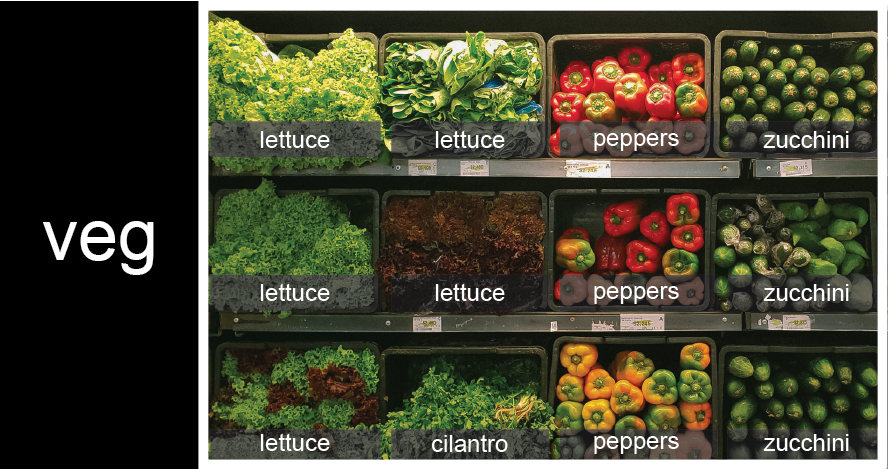
\includegraphics[keepaspectratio]{fig/04_groceries_veg.png}}

To store the contents of the shelf in a nested list, you write it this
way:

\begin{Shaded}
\begin{Highlighting}[]
\NormalTok{veg }\OperatorTok{=}\NormalTok{ [[}\StringTok{\textquotesingle{}lettuce\textquotesingle{}}\NormalTok{, }\StringTok{\textquotesingle{}lettuce\textquotesingle{}}\NormalTok{, }\StringTok{\textquotesingle{}peppers\textquotesingle{}}\NormalTok{, }\StringTok{\textquotesingle{}zucchini\textquotesingle{}}\NormalTok{],}
\NormalTok{     [}\StringTok{\textquotesingle{}lettuce\textquotesingle{}}\NormalTok{, }\StringTok{\textquotesingle{}lettuce\textquotesingle{}}\NormalTok{, }\StringTok{\textquotesingle{}peppers\textquotesingle{}}\NormalTok{, }\StringTok{\textquotesingle{}zucchini\textquotesingle{}}\NormalTok{],}
\NormalTok{     [}\StringTok{\textquotesingle{}lettuce\textquotesingle{}}\NormalTok{, }\StringTok{\textquotesingle{}cilantro\textquotesingle{}}\NormalTok{, }\StringTok{\textquotesingle{}peppers\textquotesingle{}}\NormalTok{, }\StringTok{\textquotesingle{}zucchini\textquotesingle{}}\NormalTok{]]}
\end{Highlighting}
\end{Shaded}

Here are some visual examples of how indexing a list of lists
\texttt{veg} works. First, you can reference each row on the shelf as a
separate list. For example, \texttt{veg{[}2{]}} represents the bottom
row, which is a list of the baskets in that row.

\pandocbounded{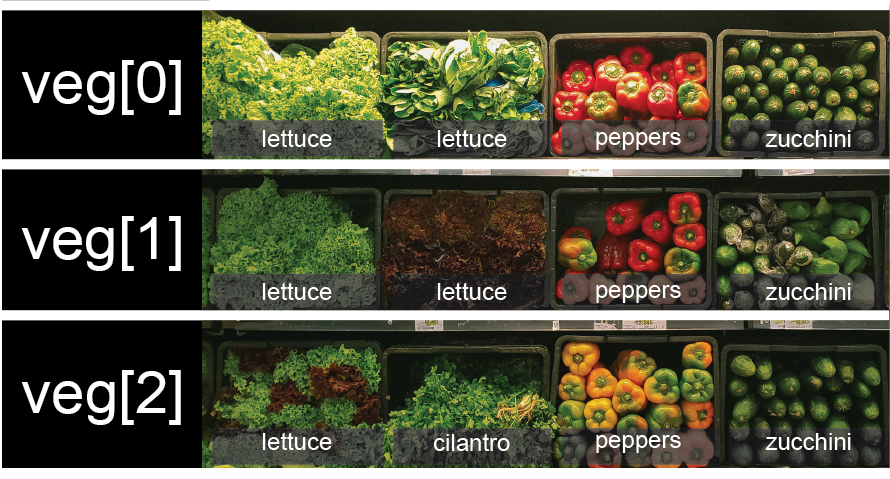
\includegraphics[keepaspectratio]{fig/04_groceries_veg0.png}}

Index operations using the image would work like this:

\begin{Shaded}
\begin{Highlighting}[]
\BuiltInTok{print}\NormalTok{(veg[}\DecValTok{2}\NormalTok{])}
\end{Highlighting}
\end{Shaded}

\begin{Shaded}
\begin{Highlighting}[]
\NormalTok{[\textquotesingle{}lettuce\textquotesingle{}, \textquotesingle{}cilantro\textquotesingle{}, \textquotesingle{}peppers\textquotesingle{}, \textquotesingle{}zucchini\textquotesingle{}]}
\end{Highlighting}
\end{Shaded}

\begin{Shaded}
\begin{Highlighting}[]
\BuiltInTok{print}\NormalTok{(veg[}\DecValTok{0}\NormalTok{])}
\end{Highlighting}
\end{Shaded}

\begin{Shaded}
\begin{Highlighting}[]
\NormalTok{[\textquotesingle{}lettuce\textquotesingle{}, \textquotesingle{}lettuce\textquotesingle{}, \textquotesingle{}peppers\textquotesingle{}, \textquotesingle{}zucchini\textquotesingle{}]}
\end{Highlighting}
\end{Shaded}

To reference a specific basket on a specific shelf, you use two indexes.
The first index represents the row (from top to bottom) and the second
index represents the specific basket (from left to right).
\pandocbounded{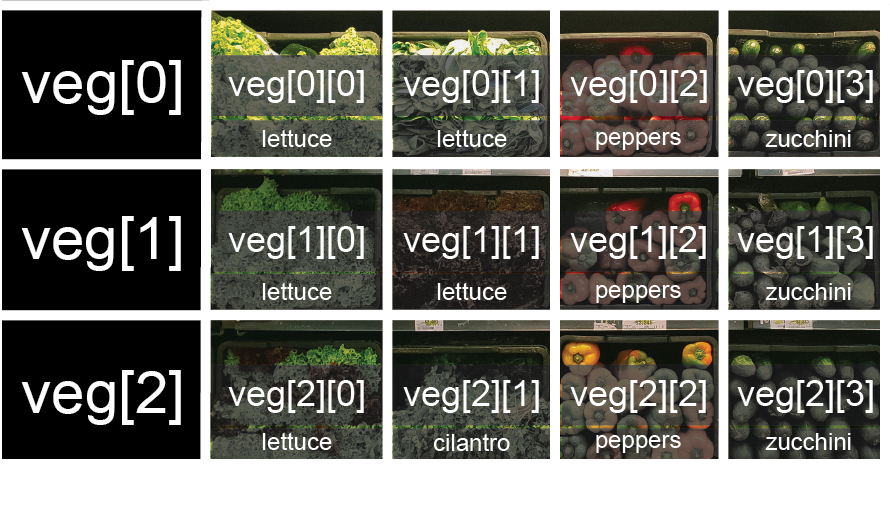
\includegraphics[keepaspectratio]{fig/04_groceries_veg00.png}}

\begin{Shaded}
\begin{Highlighting}[]
\BuiltInTok{print}\NormalTok{(veg[}\DecValTok{0}\NormalTok{][}\DecValTok{0}\NormalTok{])}
\end{Highlighting}
\end{Shaded}

\begin{Shaded}
\begin{Highlighting}[]
\NormalTok{\textquotesingle{}lettuce\textquotesingle{}}
\end{Highlighting}
\end{Shaded}

\begin{Shaded}
\begin{Highlighting}[]
\BuiltInTok{print}\NormalTok{(veg[}\DecValTok{1}\NormalTok{][}\DecValTok{2}\NormalTok{])}
\end{Highlighting}
\end{Shaded}

\begin{Shaded}
\begin{Highlighting}[]
\NormalTok{\textquotesingle{}peppers\textquotesingle{}}
\end{Highlighting}
\end{Shaded}

\end{tcolorbox}

\begin{tcolorbox}[enhanced jigsaw, bottomrule=.15mm, rightrule=.15mm, colback=white, colframe=quarto-callout-color-frame, leftrule=.75mm, arc=.35mm, breakable, toprule=.15mm, left=2mm, opacityback=0]

\vspace{-3mm}\textbf{Heterogeneous Lists}\vspace{3mm}

Lists in Python can contain elements of different types. Example:

\begin{Shaded}
\begin{Highlighting}[]
\NormalTok{sample\_ages }\OperatorTok{=}\NormalTok{ [}\DecValTok{10}\NormalTok{, }\FloatTok{12.5}\NormalTok{, }\StringTok{\textquotesingle{}Unknown\textquotesingle{}}\NormalTok{]}
\end{Highlighting}
\end{Shaded}

\end{tcolorbox}

There are many ways to change the contents of lists besides assigning
new values to individual elements:

\begin{Shaded}
\begin{Highlighting}[]
\NormalTok{odds.append(}\DecValTok{11}\NormalTok{)}
\BuiltInTok{print}\NormalTok{(}\StringTok{\textquotesingle{}odds after adding a value:\textquotesingle{}}\NormalTok{, odds)}
\end{Highlighting}
\end{Shaded}

\begin{Shaded}
\begin{Highlighting}[]
\NormalTok{odds after adding a value: [1, 3, 5, 7, 11]}
\end{Highlighting}
\end{Shaded}

\begin{Shaded}
\begin{Highlighting}[]
\NormalTok{removed\_element }\OperatorTok{=}\NormalTok{ odds.pop(}\DecValTok{0}\NormalTok{)}
\BuiltInTok{print}\NormalTok{(}\StringTok{\textquotesingle{}odds after removing the first element:\textquotesingle{}}\NormalTok{, odds)}
\BuiltInTok{print}\NormalTok{(}\StringTok{\textquotesingle{}removed\_element:\textquotesingle{}}\NormalTok{, removed\_element)}
\end{Highlighting}
\end{Shaded}

\begin{Shaded}
\begin{Highlighting}[]
\NormalTok{odds after removing the first element: [3, 5, 7, 11]}
\NormalTok{removed\_element: 1}
\end{Highlighting}
\end{Shaded}

\begin{Shaded}
\begin{Highlighting}[]
\NormalTok{odds.reverse()}
\BuiltInTok{print}\NormalTok{(}\StringTok{\textquotesingle{}odds after reversing:\textquotesingle{}}\NormalTok{, odds)}
\end{Highlighting}
\end{Shaded}

\begin{Shaded}
\begin{Highlighting}[]
\NormalTok{odds after reversing: [11, 7, 5, 3]}
\end{Highlighting}
\end{Shaded}

While modifying in place, it is useful to remember that Python treats
lists in a slightly counter-intuitive way.

As we saw earlier, when we modified the \texttt{mild\_salsa} list item
in-place, if we make a list, (attempt to) copy it and then modify this
list, we can cause all sorts of trouble. This also applies to modifying
the list using the above functions:

\begin{Shaded}
\begin{Highlighting}[]
\NormalTok{odds }\OperatorTok{=}\NormalTok{ [}\DecValTok{3}\NormalTok{, }\DecValTok{5}\NormalTok{, }\DecValTok{7}\NormalTok{]}
\NormalTok{primes }\OperatorTok{=}\NormalTok{ odds}
\NormalTok{primes.append(}\DecValTok{2}\NormalTok{)}
\BuiltInTok{print}\NormalTok{(}\StringTok{\textquotesingle{}primes:\textquotesingle{}}\NormalTok{, primes)}
\BuiltInTok{print}\NormalTok{(}\StringTok{\textquotesingle{}odds:\textquotesingle{}}\NormalTok{, odds)}
\end{Highlighting}
\end{Shaded}

\begin{Shaded}
\begin{Highlighting}[]
\NormalTok{primes: [3, 5, 7, 2]}
\NormalTok{odds: [3, 5, 7, 2]}
\end{Highlighting}
\end{Shaded}

This is because Python stores a list in memory, and then can use
multiple names to refer to the same list. If all we want to do is copy a
(simple) list, we can again use the \texttt{list} function, so we do not
modify a list we did not mean to:

\begin{Shaded}
\begin{Highlighting}[]
\NormalTok{odds }\OperatorTok{=}\NormalTok{ [}\DecValTok{3}\NormalTok{, }\DecValTok{5}\NormalTok{, }\DecValTok{7}\NormalTok{]}
\NormalTok{primes }\OperatorTok{=} \BuiltInTok{list}\NormalTok{(odds)}
\NormalTok{primes.append(}\DecValTok{2}\NormalTok{)}
\BuiltInTok{print}\NormalTok{(}\StringTok{\textquotesingle{}primes:\textquotesingle{}}\NormalTok{, primes)}
\BuiltInTok{print}\NormalTok{(}\StringTok{\textquotesingle{}odds:\textquotesingle{}}\NormalTok{, odds)}
\end{Highlighting}
\end{Shaded}

\begin{Shaded}
\begin{Highlighting}[]
\NormalTok{primes: [3, 5, 7, 2]}
\NormalTok{odds: [3, 5, 7]}
\end{Highlighting}
\end{Shaded}

Subsets of lists and strings can be accessed by specifying ranges of
values in brackets, similar to how we accessed ranges of positions in a
NumPy array. This is commonly referred to as ``slicing'' the
list/string.

\begin{Shaded}
\begin{Highlighting}[]
\NormalTok{binomial\_name }\OperatorTok{=} \StringTok{\textquotesingle{}Drosophila melanogaster\textquotesingle{}}
\NormalTok{group }\OperatorTok{=}\NormalTok{ binomial\_name[}\DecValTok{0}\NormalTok{:}\DecValTok{10}\NormalTok{]}
\BuiltInTok{print}\NormalTok{(}\StringTok{\textquotesingle{}group:\textquotesingle{}}\NormalTok{, group)}

\NormalTok{species }\OperatorTok{=}\NormalTok{ binomial\_name[}\DecValTok{11}\NormalTok{:}\DecValTok{23}\NormalTok{]}
\BuiltInTok{print}\NormalTok{(}\StringTok{\textquotesingle{}species:\textquotesingle{}}\NormalTok{, species)}

\NormalTok{chromosomes }\OperatorTok{=}\NormalTok{ [}\StringTok{\textquotesingle{}X\textquotesingle{}}\NormalTok{, }\StringTok{\textquotesingle{}Y\textquotesingle{}}\NormalTok{, }\StringTok{\textquotesingle{}2\textquotesingle{}}\NormalTok{, }\StringTok{\textquotesingle{}3\textquotesingle{}}\NormalTok{, }\StringTok{\textquotesingle{}4\textquotesingle{}}\NormalTok{]}
\NormalTok{autosomes }\OperatorTok{=}\NormalTok{ chromosomes[}\DecValTok{2}\NormalTok{:}\DecValTok{5}\NormalTok{]}
\BuiltInTok{print}\NormalTok{(}\StringTok{\textquotesingle{}autosomes:\textquotesingle{}}\NormalTok{, autosomes)}

\NormalTok{last }\OperatorTok{=}\NormalTok{ chromosomes[}\OperatorTok{{-}}\DecValTok{1}\NormalTok{]}
\BuiltInTok{print}\NormalTok{(}\StringTok{\textquotesingle{}last:\textquotesingle{}}\NormalTok{, last)}
\end{Highlighting}
\end{Shaded}

\begin{Shaded}
\begin{Highlighting}[]
\NormalTok{group: Drosophila}
\NormalTok{species: melanogaster}
\NormalTok{autosomes: [\textquotesingle{}2\textquotesingle{}, \textquotesingle{}3\textquotesingle{}, \textquotesingle{}4\textquotesingle{}]}
\NormalTok{last: 4}
\end{Highlighting}
\end{Shaded}

\subsection{Slicing From the End}\label{slicing-from-the-end}

Use slicing to access only the last four characters of a string or
entries of a list.

\begin{Shaded}
\begin{Highlighting}[]
\NormalTok{string\_for\_slicing }\OperatorTok{=} \StringTok{\textquotesingle{}Observation date: 02{-}Feb{-}2013\textquotesingle{}}
\NormalTok{list\_for\_slicing }\OperatorTok{=}\NormalTok{ [[}\StringTok{\textquotesingle{}fluorine\textquotesingle{}}\NormalTok{, }\StringTok{\textquotesingle{}F\textquotesingle{}}\NormalTok{],}
\NormalTok{                    [}\StringTok{\textquotesingle{}chlorine\textquotesingle{}}\NormalTok{, }\StringTok{\textquotesingle{}Cl\textquotesingle{}}\NormalTok{],}
\NormalTok{                    [}\StringTok{\textquotesingle{}bromine\textquotesingle{}}\NormalTok{, }\StringTok{\textquotesingle{}Br\textquotesingle{}}\NormalTok{],}
\NormalTok{                    [}\StringTok{\textquotesingle{}iodine\textquotesingle{}}\NormalTok{, }\StringTok{\textquotesingle{}I\textquotesingle{}}\NormalTok{],}
\NormalTok{                    [}\StringTok{\textquotesingle{}astatine\textquotesingle{}}\NormalTok{, }\StringTok{\textquotesingle{}At\textquotesingle{}}\NormalTok{]]}
\end{Highlighting}
\end{Shaded}

\begin{Shaded}
\begin{Highlighting}[]
\NormalTok{\textquotesingle{}2013\textquotesingle{}}
\NormalTok{[[\textquotesingle{}chlorine\textquotesingle{}, \textquotesingle{}Cl\textquotesingle{}], [\textquotesingle{}bromine\textquotesingle{}, \textquotesingle{}Br\textquotesingle{}], [\textquotesingle{}iodine\textquotesingle{}, \textquotesingle{}I\textquotesingle{}], [\textquotesingle{}astatine\textquotesingle{}, \textquotesingle{}At\textquotesingle{}]]}
\end{Highlighting}
\end{Shaded}

Would your solution work regardless of whether you knew beforehand the
length of the string or list (e.g.~if you wanted to apply the solution
to a set of lists of different lengths)? If not, try to change your
approach to make it more robust.

Hint: Remember that indices can be negative as well as positive

\begin{solution}[Solution]
Use negative indices to count elements from the end of a container (such
as list or string):

\begin{Shaded}
\begin{Highlighting}[]
\NormalTok{string\_for\_slicing[}\OperatorTok{{-}}\DecValTok{4}\NormalTok{:]}
\NormalTok{list\_for\_slicing[}\OperatorTok{{-}}\DecValTok{4}\NormalTok{:]}
\end{Highlighting}
\end{Shaded}

\end{solution}

\subsection{Non-Continuous Slices}\label{non-continuous-slices}

So far we've seen how to use slicing to take single blocks of successive
entries from a sequence. But what if we want to take a subset of entries
that aren't next to each other in the sequence?

You can achieve this by providing a third argument to the range within
the brackets, called the \emph{step size}. The example below shows how
you can take every third entry in a list:

\begin{Shaded}
\begin{Highlighting}[]
\NormalTok{primes }\OperatorTok{=}\NormalTok{ [}\DecValTok{2}\NormalTok{, }\DecValTok{3}\NormalTok{, }\DecValTok{5}\NormalTok{, }\DecValTok{7}\NormalTok{, }\DecValTok{11}\NormalTok{, }\DecValTok{13}\NormalTok{, }\DecValTok{17}\NormalTok{, }\DecValTok{19}\NormalTok{, }\DecValTok{23}\NormalTok{, }\DecValTok{29}\NormalTok{, }\DecValTok{31}\NormalTok{, }\DecValTok{37}\NormalTok{]}
\NormalTok{subset }\OperatorTok{=}\NormalTok{ primes[}\DecValTok{0}\NormalTok{:}\DecValTok{12}\NormalTok{:}\DecValTok{3}\NormalTok{]}
\BuiltInTok{print}\NormalTok{(}\StringTok{\textquotesingle{}subset\textquotesingle{}}\NormalTok{, subset)}
\end{Highlighting}
\end{Shaded}

\begin{Shaded}
\begin{Highlighting}[]
\NormalTok{subset [2, 7, 17, 29]}
\end{Highlighting}
\end{Shaded}

Notice that the slice taken begins with the first entry in the range,
followed by entries taken at equally-spaced intervals (the steps)
thereafter. If you wanted to begin the subset with the third entry, you
would need to specify that as the starting point of the sliced range:

\begin{Shaded}
\begin{Highlighting}[]
\NormalTok{primes }\OperatorTok{=}\NormalTok{ [}\DecValTok{2}\NormalTok{, }\DecValTok{3}\NormalTok{, }\DecValTok{5}\NormalTok{, }\DecValTok{7}\NormalTok{, }\DecValTok{11}\NormalTok{, }\DecValTok{13}\NormalTok{, }\DecValTok{17}\NormalTok{, }\DecValTok{19}\NormalTok{, }\DecValTok{23}\NormalTok{, }\DecValTok{29}\NormalTok{, }\DecValTok{31}\NormalTok{, }\DecValTok{37}\NormalTok{]}
\NormalTok{subset }\OperatorTok{=}\NormalTok{ primes[}\DecValTok{2}\NormalTok{:}\DecValTok{12}\NormalTok{:}\DecValTok{3}\NormalTok{]}
\BuiltInTok{print}\NormalTok{(}\StringTok{\textquotesingle{}subset\textquotesingle{}}\NormalTok{, subset)}
\end{Highlighting}
\end{Shaded}

\begin{Shaded}
\begin{Highlighting}[]
\NormalTok{subset [5, 13, 23, 37]}
\end{Highlighting}
\end{Shaded}

Use the step size argument to create a new string that contains only
every other character in the string ``In an octopus's garden in the
shade''. Start with creating a variable to hold the string:

\begin{Shaded}
\begin{Highlighting}[]
\NormalTok{beatles }\OperatorTok{=} \StringTok{"In an octopus\textquotesingle{}s garden in the shade"}
\end{Highlighting}
\end{Shaded}

What slice of \texttt{beatles} will produce the following output (i.e.,
the first character, third character, and every other character through
the end of the string)?

\begin{Shaded}
\begin{Highlighting}[]
\NormalTok{I notpssgre ntesae}
\end{Highlighting}
\end{Shaded}

\begin{solution}[Solution]
To obtain every other character you need to provide a slice with the
step size of 2:

\begin{Shaded}
\begin{Highlighting}[]
\NormalTok{beatles[}\DecValTok{0}\NormalTok{:}\DecValTok{35}\NormalTok{:}\DecValTok{2}\NormalTok{]}
\end{Highlighting}
\end{Shaded}

You can also leave out the beginning and end of the slice to take the
whole string and provide only the step argument to go every second
element:

\begin{Shaded}
\begin{Highlighting}[]
\NormalTok{beatles[::}\DecValTok{2}\NormalTok{]}
\end{Highlighting}
\end{Shaded}

\end{solution}

If you want to take a slice from the beginning of a sequence, you can
omit the first index in the range:

\begin{Shaded}
\begin{Highlighting}[]
\NormalTok{date }\OperatorTok{=} \StringTok{\textquotesingle{}Monday 4 January 2016\textquotesingle{}}
\NormalTok{day }\OperatorTok{=}\NormalTok{ date[}\DecValTok{0}\NormalTok{:}\DecValTok{6}\NormalTok{]}
\BuiltInTok{print}\NormalTok{(}\StringTok{\textquotesingle{}Using 0 to begin range:\textquotesingle{}}\NormalTok{, day)}
\NormalTok{day }\OperatorTok{=}\NormalTok{ date[:}\DecValTok{6}\NormalTok{]}
\BuiltInTok{print}\NormalTok{(}\StringTok{\textquotesingle{}Omitting beginning index:\textquotesingle{}}\NormalTok{, day)}
\end{Highlighting}
\end{Shaded}

\begin{Shaded}
\begin{Highlighting}[]
\NormalTok{Using 0 to begin range: Monday}
\NormalTok{Omitting beginning index: Monday}
\end{Highlighting}
\end{Shaded}

And similarly, you can omit the ending index in the range to take a
slice to the very end of the sequence:

\begin{Shaded}
\begin{Highlighting}[]
\NormalTok{months }\OperatorTok{=}\NormalTok{ [}\StringTok{\textquotesingle{}jan\textquotesingle{}}\NormalTok{, }\StringTok{\textquotesingle{}feb\textquotesingle{}}\NormalTok{, }\StringTok{\textquotesingle{}mar\textquotesingle{}}\NormalTok{, }\StringTok{\textquotesingle{}apr\textquotesingle{}}\NormalTok{, }\StringTok{\textquotesingle{}may\textquotesingle{}}\NormalTok{, }\StringTok{\textquotesingle{}jun\textquotesingle{}}\NormalTok{, }\StringTok{\textquotesingle{}jul\textquotesingle{}}\NormalTok{, }\StringTok{\textquotesingle{}aug\textquotesingle{}}\NormalTok{, }\StringTok{\textquotesingle{}sep\textquotesingle{}}\NormalTok{, }\StringTok{\textquotesingle{}oct\textquotesingle{}}\NormalTok{, }\StringTok{\textquotesingle{}nov\textquotesingle{}}\NormalTok{, }\StringTok{\textquotesingle{}dec\textquotesingle{}}\NormalTok{]}
\NormalTok{sond }\OperatorTok{=}\NormalTok{ months[}\DecValTok{8}\NormalTok{:}\DecValTok{12}\NormalTok{]}
\BuiltInTok{print}\NormalTok{(}\StringTok{\textquotesingle{}With known last position:\textquotesingle{}}\NormalTok{, sond)}
\NormalTok{sond }\OperatorTok{=}\NormalTok{ months[}\DecValTok{8}\NormalTok{:}\BuiltInTok{len}\NormalTok{(months)]}
\BuiltInTok{print}\NormalTok{(}\StringTok{\textquotesingle{}Using len() to get last entry:\textquotesingle{}}\NormalTok{, sond)}
\NormalTok{sond }\OperatorTok{=}\NormalTok{ months[}\DecValTok{8}\NormalTok{:]}
\BuiltInTok{print}\NormalTok{(}\StringTok{\textquotesingle{}Omitting ending index:\textquotesingle{}}\NormalTok{, sond)}
\end{Highlighting}
\end{Shaded}

\begin{Shaded}
\begin{Highlighting}[]
\NormalTok{With known last position: [\textquotesingle{}sep\textquotesingle{}, \textquotesingle{}oct\textquotesingle{}, \textquotesingle{}nov\textquotesingle{}, \textquotesingle{}dec\textquotesingle{}]}
\NormalTok{Using len() to get last entry: [\textquotesingle{}sep\textquotesingle{}, \textquotesingle{}oct\textquotesingle{}, \textquotesingle{}nov\textquotesingle{}, \textquotesingle{}dec\textquotesingle{}]}
\NormalTok{Omitting ending index: [\textquotesingle{}sep\textquotesingle{}, \textquotesingle{}oct\textquotesingle{}, \textquotesingle{}nov\textquotesingle{}, \textquotesingle{}dec\textquotesingle{}]}
\end{Highlighting}
\end{Shaded}

\subsection{Overloading}\label{overloading}

\texttt{+} usually means addition, but when used on strings or lists, it
means ``concatenate''. Given that, what do you think the multiplication
operator \texttt{*} does on lists? In particular, what will be the
output of the following code?

\begin{Shaded}
\begin{Highlighting}[]
\NormalTok{counts }\OperatorTok{=}\NormalTok{ [}\DecValTok{2}\NormalTok{, }\DecValTok{4}\NormalTok{, }\DecValTok{6}\NormalTok{, }\DecValTok{8}\NormalTok{, }\DecValTok{10}\NormalTok{]}
\NormalTok{repeats }\OperatorTok{=}\NormalTok{ counts }\OperatorTok{*} \DecValTok{2}
\BuiltInTok{print}\NormalTok{(repeats)}
\end{Highlighting}
\end{Shaded}

\begin{enumerate}
\def\labelenumi{\arabic{enumi}.}
\tightlist
\item
  \texttt{{[}2,\ 4,\ 6,\ 8,\ 10,\ 2,\ 4,\ 6,\ 8,\ 10{]}}
\item
  \texttt{{[}4,\ 8,\ 12,\ 16,\ 20{]}}
\item
  \texttt{{[}{[}2,\ 4,\ 6,\ 8,\ 10{]},\ {[}2,\ 4,\ 6,\ 8,\ 10{]}{]}}
\item
  \texttt{{[}2,\ 4,\ 6,\ 8,\ 10,\ 4,\ 8,\ 12,\ 16,\ 20{]}}
\end{enumerate}

The technical term for this is \emph{operator overloading}: a single
operator, like \texttt{+} or \texttt{*}, can do different things
depending on what it's applied to.

\begin{solution}[Solution]
The multiplication operator \texttt{*} used on a list replicates
elements of the list and concatenates them together:

\begin{Shaded}
\begin{Highlighting}[]
\NormalTok{[2, 4, 6, 8, 10, 2, 4, 6, 8, 10]}
\end{Highlighting}
\end{Shaded}

It's equivalent to:

\begin{Shaded}
\begin{Highlighting}[]
\NormalTok{counts }\OperatorTok{+}\NormalTok{ counts}
\end{Highlighting}
\end{Shaded}

\end{solution}

\begin{itemize}
\tightlist
\item
  \texttt{{[}value1,\ value2,\ value3,\ ...{]}} creates a list.
\item
  Lists can contain any Python object, including lists (i.e., list of
  lists).
\item
  Lists are indexed and sliced with square brackets (e.g.,
  \texttt{list{[}0{]}} and \texttt{list{[}2:9{]}}), in the same way as
  strings and arrays.
\item
  Lists are mutable (i.e., their values can be changed in place).
\item
  Strings are immutable (i.e., the characters in them cannot be
  changed).
\end{itemize}




\end{document}
